\documentclass{article}

\usepackage{floatrow}
\usepackage{graphicx} % Required for inserting images
\usepackage[a4paper, total={6in, 8in}]{geometry}
\usepackage{parskip} % Required to stop indenting new paragraphs
\usepackage{amssymb}
\usepackage{amsmath}
\usepackage{algpseudocode}
\usepackage{algorithm}
\usepackage[numbers]{natbib} % number references and natbib for more styles
\bibliographystyle{unsrtnat} % sets bibliography to vancouver style

\title{Rough notes/work to put in project}
\date{}

\begin{document}

\maketitle
\tableofcontents
\newpage

\section{Algorithm Dump}

\begin{algorithm}
\caption{Evaluate Postvisitor}\label{evalpostvisitor}
\begin{algorithmic}[1]
\Procedure{Euclid}{$expr,conditions$}\Comment{Expression and conditions}
\State $stack = []$
\State $visited = \{\}$
\State Push $expr$ onto $stack$
\While{$stack$ is not empty}
\State $element \gets stack.pop()$
\For{$operand \in element.opernads$}
\If{$operand \not \in visited$}
\State $unvisited\_children.push(operand)$
\EndIf
\EndFor
\If{$unvisited\_children not empty$}
\State $stack.push(element)$
\State $stack.push(unvisited\_children)$
\Else
\State $visited[element] \gets$ evaluate$(element, *(visited[operand]$ for $operand$ in $element.opernads), symbol\_map = conditions)$
\State $element.storedvalue \gets visited[element]$
\EndIf
\EndWhile\label{euclidendwhile}
\State \textbf{return} $visited[expr]$
\EndProcedure
\end{algorithmic}
\end{algorithm}


Algorithm \ref{EvaluatePostvisitor} provides the pseudocode behind the \verb|EvaluatePostvisitor| function. This will traverse through the tree in postorder and evaluate each node as it goes along. The \verb|evaluate| function for a node itself will depend on the \verb|type()| of node (what its operators are), its already evaluated operands, and the initial conditions. For example \verb|Add(x, y)| with initial conditions \verb|x = 2, y = 3| will be evaluated by evaluating \verb|x| and \verb|y| first, which will both \verb|x.storedvalue = 2| and \verb|y.storedvalue = 3|. Then \verb|Add(x, y)| will be evaluated and \verb|Add(x, y).storedvalue() = 5|. Finally, the function will return $5$
\\\\
Using the graph below we can see what our function looks like after our EvaluatePostvisitor function.
\\\\
Next Algorithm \ref{AdjointPrevisitor} provides the pseudocode behind the \verb|AdjointPrevisitor()| function, this will now traverse through the tree in preorder, evaluating the adjoints of the operands of the node as it goes along. This different \verb|evaluate_adjoint| function for a node itself will depend on the \verb|type()| of node (what its operators are), and the \verb|storedvalue| for its operands. Once this function has evaluated the adjoint of an operand, it will recursively call itself again on its operand, this allows us to do preorder traversal on our expression tree.
\\\\
Using the graph below we can see what our function looks like after our AdjointPrevisitor function.
\\\\
Next Algorithm \ref{forwardAD} provides the pseudocode behind the \verb|ReversemodeAD()| which takes in \verb|expression| and \verb|conditions| which are the expression and conditions to evaluate the derivative at and returns a dictionary of the partial derivatives of \verb|expression| w.r.t. the symbols in \verb|expression|. It does this by simply running our \verb|EvaluatePostvisitor(expression, conditions)|. And then running \verb|AdjointPrevisitor(expression)|. Once both are run we now have adjoints attached to every node/element in expression. It will then return a dictionary of the symbols and their respective adjoints (which are the partial derivatives)


\begin{algorithm}
\caption{ForwardmodeAD algorithm}\label{forwardAD}
\begin{algorithmic}[1]
\Procedure{ForwardmodeAD}{$expression,conditions$}
\State dict = dict()
\For{ each symbol in conditions}
\State non recursively traverse through $expression$, visiting $element$ after its $operands$
    \For{ each \verb|element| in expression}
    \State set \verb|element.adjoint = 0|\Comment{So we don't use adjoints calculated for other symbols}
    \State evaluate value and \verb|adjoint| of \verb|element| w.r.t. its \verb|type()|, \verb|operands| and \verb|symbol|
    \State dict[symbol] = \verb|expression.adjoint|\Comment{Store the adjoint w.r.t the symbol}
    \EndFor
\EndFor
\State \textbf{return} a dictionary of symbols and their respective \verb|adjoints|
\EndProcedure
\end{algorithmic}
\end{algorithm}



\section{Dump 2}

If $n=m=1$ then
\begin{equation*}
    f'(x) \approx \frac{f(x+h)-f(x)}{h}
\end{equation*}
and from \cite{quarteroni} it is known that
\begin{equation*}
    f'(x) - \frac{f(x+h)-f(x)}{h} = - \frac{h}{2} f''(\xi)
\end{equation*}
where $\xi \in (x, x+h)$.

\textbf{REFERENCE: https://rufflewind.com/2016-12-30/reverse-mode-automatic-differentiation}



\section{Removed sections}


Reverse mode AD consists of a forward pass over the expression tree followed by a reverse pass. The forward pass starts by substituting values into the independent variable(s) and then using these to evaluate the expressions of their parent node(s). This process propagates up the tree to the dependent variable(s). At each node, the evaluation is stored to be used in the reverse pass.

During the reverse pass, the adjoint values of each node, $\bar{w_i} = \frac{\partial{y}}{\partial{w_i}}$, are calculated using the expression:

\begin{equation}
\Bar{v_i} = \sum_{j\in\{\mbox{parent of i}\}} \Bar{v_j}\frac{\partial{v_j}}{\partial{v_i}}
\end{equation}

In the following example, we find the derivative of the function $J = xsin(x+y)$ with respect to the variables $x$ and $y$ when $(x, y) = (1, 1)$.

First, the nodes in the expression tree are labeled in the following way:
\begin{equation}
w_1 = x
\end{equation}
\begin{equation}
w_2 = y
\end{equation}
\begin{equation}
w_3 = w_1 + w_2
\end{equation}
\begin{equation}
w_4 = sin(w_3)
\end{equation}
\begin{equation}
w_5 = w_1 \cdot w_4
\end{equation}
\\\\

Suppose we want to compute $\frac{\partial{J}}{\partial{u}}$ with $u = (x, y) = (1, 1)$, performing the forward pass we obtain $w_1 = 1, w_2 = 1, w_3 = 2, w_4 = sin(2), w_5 = sin(2)$.

For the reverse pass, we seed the value of $\bar{w_5}$ as 1 then, using the formula for $\bar{w_i}$, we obtain:
\begin{equation}
\bar{w_4} = \bar{w_5}\frac{\partial{w_5}}{\partial{w_4}} = \bar{w_5}\cdot w_1 = 1
\end{equation}
\begin{equation}
\bar{w_3} = \bar{w_4}\frac{\partial{w_4}}{\partial{w_3}} = \bar{w_4}\cdot cos(w_3) = cos(2)
\end{equation}
\begin{equation}
\bar{w_2} = \bar{w_3}\frac{\partial{w_3}}{\partial{w_2}} = \bar{w_3}\cdot w_1 = cos(2)
\end{equation}
\begin{equation}
\bar{w_1} = \bar{w_5}\frac{\partial{w_5}}{\partial{w_1}} + \bar{w_3}\frac{\partial{w_3}}{\partial{w_1}} = \bar{w_5}\cdot w_4 + \bar{w_3} = sin(2) + cos(2)
\end{equation}
Therefore, we have computed $\frac{\partial{J}}{\partial{x}}\vert_{(1, 1)} = sin(2) + cos(2)$ and $\frac{\partial{J}}{\partial{y}}\vert_{(1, 1)} = cos(2)$.



\begin{center}
    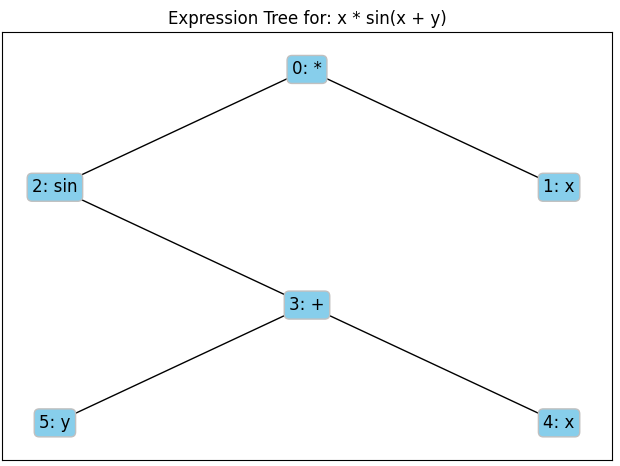
\includegraphics[width=12cm]{images/DAG_1.png}
\end{center}

Now we have the graph, we can operate a forward pass and at each node, we save the value outputted. Taking the example $x = 1$ and $y = 1$ we assign values to nodes as so:

\begin{equation*}
    5: (1, ) 
\end{equation*}
\begin{equation*}
    4: (1, )
\end{equation*}
\begin{equation*}
    3: (2, )
\end{equation*}
\begin{equation*}
    2: (0.90929, )
\end{equation*}
\begin{equation*}
    1: (1, )
\end{equation*}
\begin{equation*}
    0: (0.90929, )
\end{equation*}

Here we are numbering the nodes as they have been in the graph. Having computed these in the first pass we then, using equations (14) - (18) stated above we now calculate the adjoint values by doing a backward pass and assigning them to each node as so:

\begin{equation*}
    5: (1, -0.41615)
\end{equation*}
\begin{equation*}
    4: (1, 0.49315)
\end{equation*}
\begin{equation*}
    3: (2, -0.41615)
\end{equation*}
\begin{equation*}
    2: (0.90929, 1)
\end{equation*}
\begin{equation*}
    1: (1, 0.90929)
\end{equation*}
\begin{equation*}
    0: (0.90929, 1)
\end{equation*}

Returning these values we see that our $\frac{dJ}{dx} = 0.49315 = cos(2) + sin(2)$ is the adjoint value of the x node (node 4) and our $\frac{dJ}{dy} = -0.41615 = cos(2)$ is the adjoint value of the y node (node 5).

The expression was then broken down into the elementary functions ($+, -, *, /, sin, cos, exp, log$), from there we define a Directed Acyclic Graph using the earlier elementary functions and parent nodes and the one that follows child nodes, using network x to represent this we can represent (18) by the graph:


\section{Testing image and table side by side}

\begin{figure}[h!]
\begin{floatrow}
\ffigbox{%
  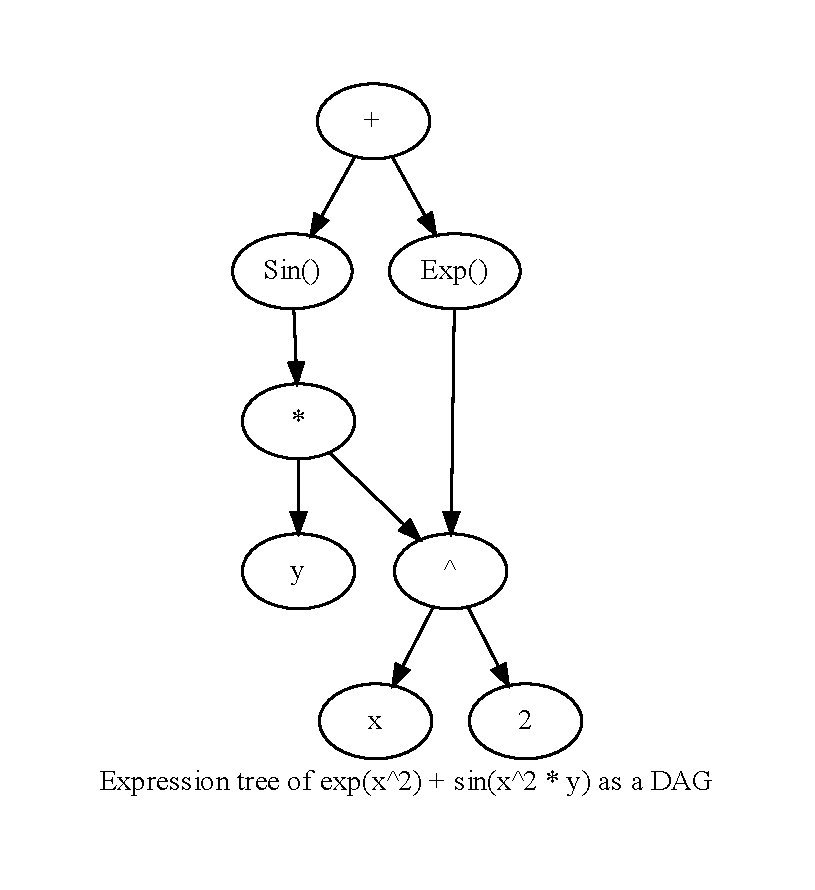
\includegraphics[width=5cm]{images/DAGgraph.gv.pdf}
}{%
}
\capbtabbox{%
  \begin{tabular}{|lcl|lclll|}
        \hline
        $v_{-1}$ & $\equiv$ & $x$ & $\Bar{v}_{-1}$ & $\equiv$ & $\Bar{v_2}\frac{\partial{v_2}}{\partial{v_{-1}}}$ & $=$ & $\Bar{v_2}v_1 {v_{-1}}^{(v_{1}-1)}$\\
        $v_{0}$ & $\equiv$ & $y$ & $\Bar{v}_{0}$ & $\equiv$ & $\Bar{v_3}\frac{\partial{v_3}}{\partial{v_0}}$ & $=$ & $\Bar{v_3}v_2$\\
        \hline
        $v_{1}$ & $\equiv$ & $2$ & $\Bar{v}_{1}$ & $\equiv$ & $\Bar{v_2}\frac{\partial{v_2}}{\partial{v_1}}$ & $=$ & $\Bar{v}_{2}{v_{-1}}^{v_{1}}ln(v_{-1})$\\
        $v_{2}$ & $\equiv$ & ${v_{-1}}^{v_{1}}$ & $\Bar{v}_{2}$ & $\equiv$ & $\Bar{v_3}\frac{\partial{v_3}}{\partial{v_2}} + \Bar{v_5}\frac{\partial{v_5}}{\partial{v_2}}$ & $=$ & $\Bar{v}_{3}v_0 + \Bar{v_5}e^{v_2}$\\
        $v_{3}$ & $\equiv$ & ${v_{0}}*{v_{2}}$ & $\Bar{v}_{3}$ & $\equiv$ & $\Bar{v_4}\frac{\partial{v_4}}{\partial{v_3}}$ & $=$ & $\Bar{v_4}cos(v_2)$\\
        $v_{4}$ & $\equiv$ & $sin(v_3)$ & $\Bar{v}_{4}$ & $\equiv$ & $\Bar{v_6}\frac{\partial{v_6}}{\partial{v_4}}$ & $=$ & $\Bar{v_6}$\\
        $v_{5}$ & $\equiv$ & $e^{v_2}$ & $\Bar{v}_{5}$ & $\equiv$ & $\Bar{v_6}\frac{\partial{v_6}}{\partial{v_5}}$ & $=$ & $\Bar{v_6}$\\
        \hline
        $v_{6}$ & $\equiv$ & $v_5 + v_4$ & $\Bar{v}_{6}$ & $\equiv$ & $\frac{\partial{v_6}}{\partial{v_6}}$ & $=$ & $1$\\
        \hline
    \end{tabular}
}{%
  \caption{Table of nodes in Figure 2 of Equation 7}%
}
\end{floatrow}
\end{figure}





\end{document}